\chapter{Introduzione}
In questo capitolo verranno esposte le motivazioni e gli obbiettivi di questo lavoro, a partire dalla situazione odierna per descriverne i problemi che hanno portato allo sviluppo dello standard IEEE 802.21.

\section{La situazione odierna}
Il mondo di oggi è in continua evoluzione, ogni giorno abbiamo nuovi dispositivi con hardware sempre migliore non solo sotto un punto di vista qualitativo, bensì anche quantitativo, nel senso che i nuovi {\em devices} hanno sempre più elettronica a bordo per poter sfruttare le nuove tecnologie, in particolare riguardo alla connettività, diventata negli ultimi anni un aspetto fondamentale della vita di tutti i giorni. Il fatto che ormai la maggioranza dei nuovi dispositivi sia dotata di più interfacce di rete spiana la strada a molte opportunità, ma, allo stesso tempo, pone anche degli ostacoli lungo il cammino.
Chiunque possieda uno smartphone recente può connettersi alla rete in più modi, come Wi-Fi, GSM, UMTS, HSDPA, LTE, etc. Se, per esempio, siamo attualmente connessi tramite una connessione wireless ed usciamo dalla zona di copertura dell'{\em Access Point}, il {\em device} si collegherà automaticamente attraverso un'altra tecnologia, attivando le ricetrasmittenti adatte oppure se usciamo dalla zona di copertura della nostra attuale connessione GSM, il dispositivo si connetterà autonomamente ad un'altra torretta. L'atto di cambiare l'{\em access point} oppure addirittura la tecnologia utilizzata per ristabilire la connessione è detto {\em handover} e può essere più tipi. La figura \ref{fig:handovers} riassume graficamente quanto detto, mostrando i movimenti di un apparato mobile dotato di connettività Wi-Fi, WiMaX e 3G che, uscendo di volta in volta dal raggio di azione dell'{\em Access Point} a cui è attualmente connesso, adotta le azioni di {\em handover} necessarie per ripristinare la connettività, ristabilendo la connessione sull'interfaccia migliore tenendo conto delle prestazioni del {\em link} ed il consumo energetico associato.

\begin{figure}[h!]
\centering
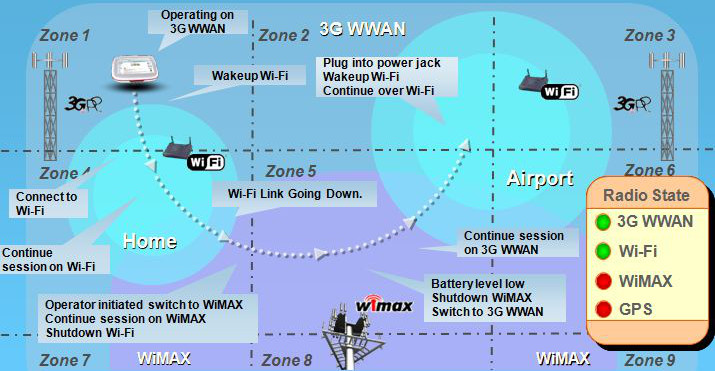
\includegraphics[scale=0.55]{handovers.jpg}
\caption{Handovers}
\label{fig:handovers}
\end{figure}

\section{Tipi di handovers}

I due esempi sopra citati descrivono rispettivamente uno scenario di {\em handover} verticale ed orizzontale, a seconda della tecnologia utilizzata prima e dopo il passaggio. Oltre a questo classificazione, è possibile descrivere altri due tipi di {\em handover}, a seconda che le connessioni aperte al momento del passaggio vengano o meno preservate nel passaggio.

\subsection{Horizontal handover}
Nel caso del telefonino che cambia la propria BTS\footnote{Base Transceiver Station}, quando esce dal raggio di azione della prima, si parla di un {\em handover} orizzontale, i.e. la tecnologia adoperata a livello {\em data link} non cambia. Stesso tipologia di {\em handover} se, muovendoci, ci si collega man mano agli {\em access points} Wi-Fi con miglior ricezione e ciò può anche essere effettuato utilizzando due interfacce 802.11 contemporaneamente in modo da avere potenzialmente entrambe le connessioni attive al momento del passaggio.

\subsection{Vertical handover}
Se è necessario, invece, cambiare il livello {\em data link} durante il passaggio, allora si tratta di un {\em handover} verticale. Sono i più utili da un punto di vista applicativo poiché permettono di sfruttare le diverse caratteristiche intrinseche di ogni particolare tecnologia, ovvero si potrebbe essere interessati ad utilizzare una connessione Wi-Fi qualora disponibile e passare su HSDPA solo quando si esce dalla zona di copertura dell'attuale {\em access point}, in modo da poter mantenere attiva la connessione, anche cambiando il mezzo trasmissivo e, di conseguenza, il livello {\em data link}.

\subsection{Hard handover}
Si tratta di un {\em handover} dove le connessioni attive prima del passaggio vengono chiuse, incaricando il dispositivo stesso di ripristinarle da zero successivamente, quando avrà stabilito con successo un nuovo collegamento. Viene anche definito come {\em break-before-make}.

\subsection{Soft handover}
In questo caso le connessioni aperte vengono mantenute anche dopo il passaggio, in modo da preservare lo stato della rete e consentire un passaggio trasparente ed indolore all'utente. Questo è realizzato stabilendo una connessione verso il nuovo {\em access point} preventivamente, in modo che, prima che il collegamento salti, si abbia già un altro canale pronto all'uso. Viene anche definito come {\em make-before-break}.

\section{Problematiche}
I problemi principali da gestire sono:
\begin{enumerate}
\item come e quando debbano effettuarsi le decisioni di {\em handover}.
\item come debba avvenire effettivamente il passaggio tra {\em access points} della stessa rete, al fine di mantenere lo stato della sessione.
\item come debba avvenire effettivamente il passaggio tra {\em access points} di reti diverse, al fine di mantenere lo stato della sessione.
\end{enumerate}
Lo standard IEEE 802.21, preso in esame in questo lavoro, mira a risolvere il primo problema, fornendo dei servizi {\em media-independent} per prendere le dovute decisioni di {\em handover} in un modo standardizzato ed indipendente dalla tecnologia utilizzata al momento, ma non stabilisce come effettivamente debba avvenire il passaggio.
Per il secondo problema è necessario stabilire opportune specifiche di come debba effettivamente avvenire l'{\em handover} tra {\em access points} della stessa rete, ad esempio come lo standard IEEE 802.11r-2008\cite{ieee80211r} per il passaggio da un {\em access point} Wi-Fi all'altro.
Per il terzo problema è possibile adottare soluzioni come il {\em Mobile IP}\cite{mobileip} dell'IETF\footnote{Internet Engineering Task Force}, il quale permette il {\em routing} dei pacchetti indipendentemente dalla posizione fisica del {\em device} associandogli un indirizzo IP permanente.